\section{Introductory thoughts}
ADflow started its life in the early 2000s and was called \textit{Standford
University Multiblock (sumb)}. It was intended for turbomachinery but was
extended for optimization later on. This extension required quite a
substantial change to the solvers structure which rendered multiple features
non working. The SST turbulence model is such a part that once worked but does
not anymore.

ADflow is written in FORTRAN, but has a python wrapper. This means, the heavy
lifting is done in a fast, compiled language, but the user has the benefits of
an interpreted, object oriented programming environment. As explained in
section \ref{sec:gradient_computation}, the adjoint method needs partial
derivatives that are (in ADflow) obtained through means of
automatic/algorithmic differentiation (AD). For this, a tool called
\textit{tapenade}
\footnote{\url{http://www-tapenade.inria.fr:8080/tapenade/index.jsp}} is used.
It automatically differentiates FORTRAN source code.

Please note it was not possible to properly cite all the ADflow specific
information given in this section. Most of it comes from talks with one of the
supervisors and developer of ADflow \textit{Dr. Anil Yildirim}. The remaining
part comes from reading the source code.




\subsection{Terms}
The following lines explain some concepts that might not be known.

\paragraph{Flow variables} Those are the variables that the solver solves for.
The state variables of the turbulence model are excluded. Here, this means:
\textit{velocity (x, y, z)}, \textit{density} and \textit{energy}.

\paragraph{Turbulence variables} The variables the solver solves for for the
turbulence. For SST, this is $k$ and $\omega$.

\paragraph{Coupled turbulence} When the turbulence variables are solved in a
coupled manner, we have only one system of equations for all variables. When
they are solved in a decoupled manner, we have two different systems: one for
the \textit{flow variables} and one for the \textit{turbulence variables}. As
everything is related to each other, solving a decoupled system slows down
convergence, but it increases robustness.




\subsection{Flow Solvers}
\label{sec:flow_solvers}
Before diving deep into the changes that made SST run, we need to understand
how ADflow solves the RANS equations and what it needs for that.

ADflow has three different solvers available: \textit{multigrid (MG)},
\textit{Newton-Krylov (NK)} and \textit{Approximate Newton-Krylov (ANK)}. It is
possible to switch between the different solvers during a solution run. This
allows to use each solver when it is most efficient. An example run might look
like: initiate the simulation using multigrid, once a certain level of
convergence is reached, engage the ANK solver and finally converge the last
couple order of magnitudes using the NK Solver. \footnote{Please note that the
ANK solver by itself is sufficient as a startup strategy and MG is not
necessarily needed.}

\paragraph{Multigrid} is the baseline solver that was implemented first. It
uses either the \textit{Runge-Kutta (RK)}, or the \textit{Diagonalized
Diagonally-Dominant Alternating Direction Implicit (D3ADI)} algorithm as a
smoother. The flow and turbulence model is solved in a decoupled manner and
using the \textit{Diagonalized Alternating Direction Implicit (DADI)} method.

\paragraph{The Newton-Krylov} solver solves the nonlinear system of governing
equations by means of Newton's method (sec. \ref{sec:newtons_method}). To solve
the linear system at each step, the GMRES\footnote{This stands for
\textit{generalized minimal residual method}.} algorithm is used. The
turbulence variables are solved in a coupled manner and thus no other solvers
are needed. This method is equivalent to using Euler's method with an infinite
time step. It is most efficient when the solution is already at the final
stages of convergence. If it is used in the early stages, it most likely
stalls.

\paragraph{The Approximate Newton-Krylov} is similar to the NK solver in that
it also uses Newton's method. But its time step is adjustable. At the beginning
of the run, it is quite low. As the solution accuracy increases, the timestep
is increased as well. This increases robustness early on but also accelerates
convergence later that would otherwise slow down drastically. The solver itself
is subdivided into three different sub-solvers: \textit{First order ANK (ANK)},
\textit{Second Order ANK (SANK)} and \textit{Coupled ANK (CANK)}. Please note,
the combination of both \textit{Coupled Second-Order ANK (CSANK)} is also
possible.

In its base configuration \textbf{ANK} uses a first-order routine for the
residual Jacobian where as the second order formulation \textbf{SANK} is as
accurate as ADflows discretization is. The idea of this solver is to solve only
as much as needed. In that context, it makes sense to use the first-order
formulation early on when the solution is far from convergence. This not only
saves computing power but also increases convergence because high frequency
oscillations may not be captured. Once a user defined level of convergence is
reached, the solver switches to an exact Jacobian formulation (SANK). 

In these first two stages, the turbulence model is solved in a decoupled manner
using either a second, turbulence specifi ANK solver (from now on called
\textit{ANK-turb}) or a legacy \textit{Diagonalized Alternating Direction
Implicit (DADI)} method. Splitting it up is beneficial early on as it increases
robustness. Once again, when the residual norm reaches a user-defined level,
the coupled mode (\textbf{CANK}) is engaged. In that state, only one ANK
solver remains which solves the flow and turbulence variables simultaneously.
This helps to improve the convergence in the later stages.
\cite{adflow_solvers}

The ANK solver is made even more robust by introducing the concept of a
\textit{physicality check}. When looking at section \ref{sec:newtons_method},
we see that we need to solve a linear system to obtain the next newton step.
The solution of this system does not only depend on the accuracy of our residual
computation but also on how accurate we solve the linear system. This means, a
step we obtain might actually lead to a divergence of the solution. To  prevent
this, the ANK solver performs some checks to make sure the current step
improves the solution. If this is not the case, it tries to apply only part of
the step \footnote{This concept is known as backtracking.}.




\subsection{Adjoint Solver and total derivatives}
\label{subsec:adjoint}
When computing the total derivatives, it is important to realize that the
adjoint solver is not the whole story. Take a look at figure \ref{fig:MACH}. It
shows the flow of data for a simple airfoil optimization example.

\begin{figure}[H] \centering
    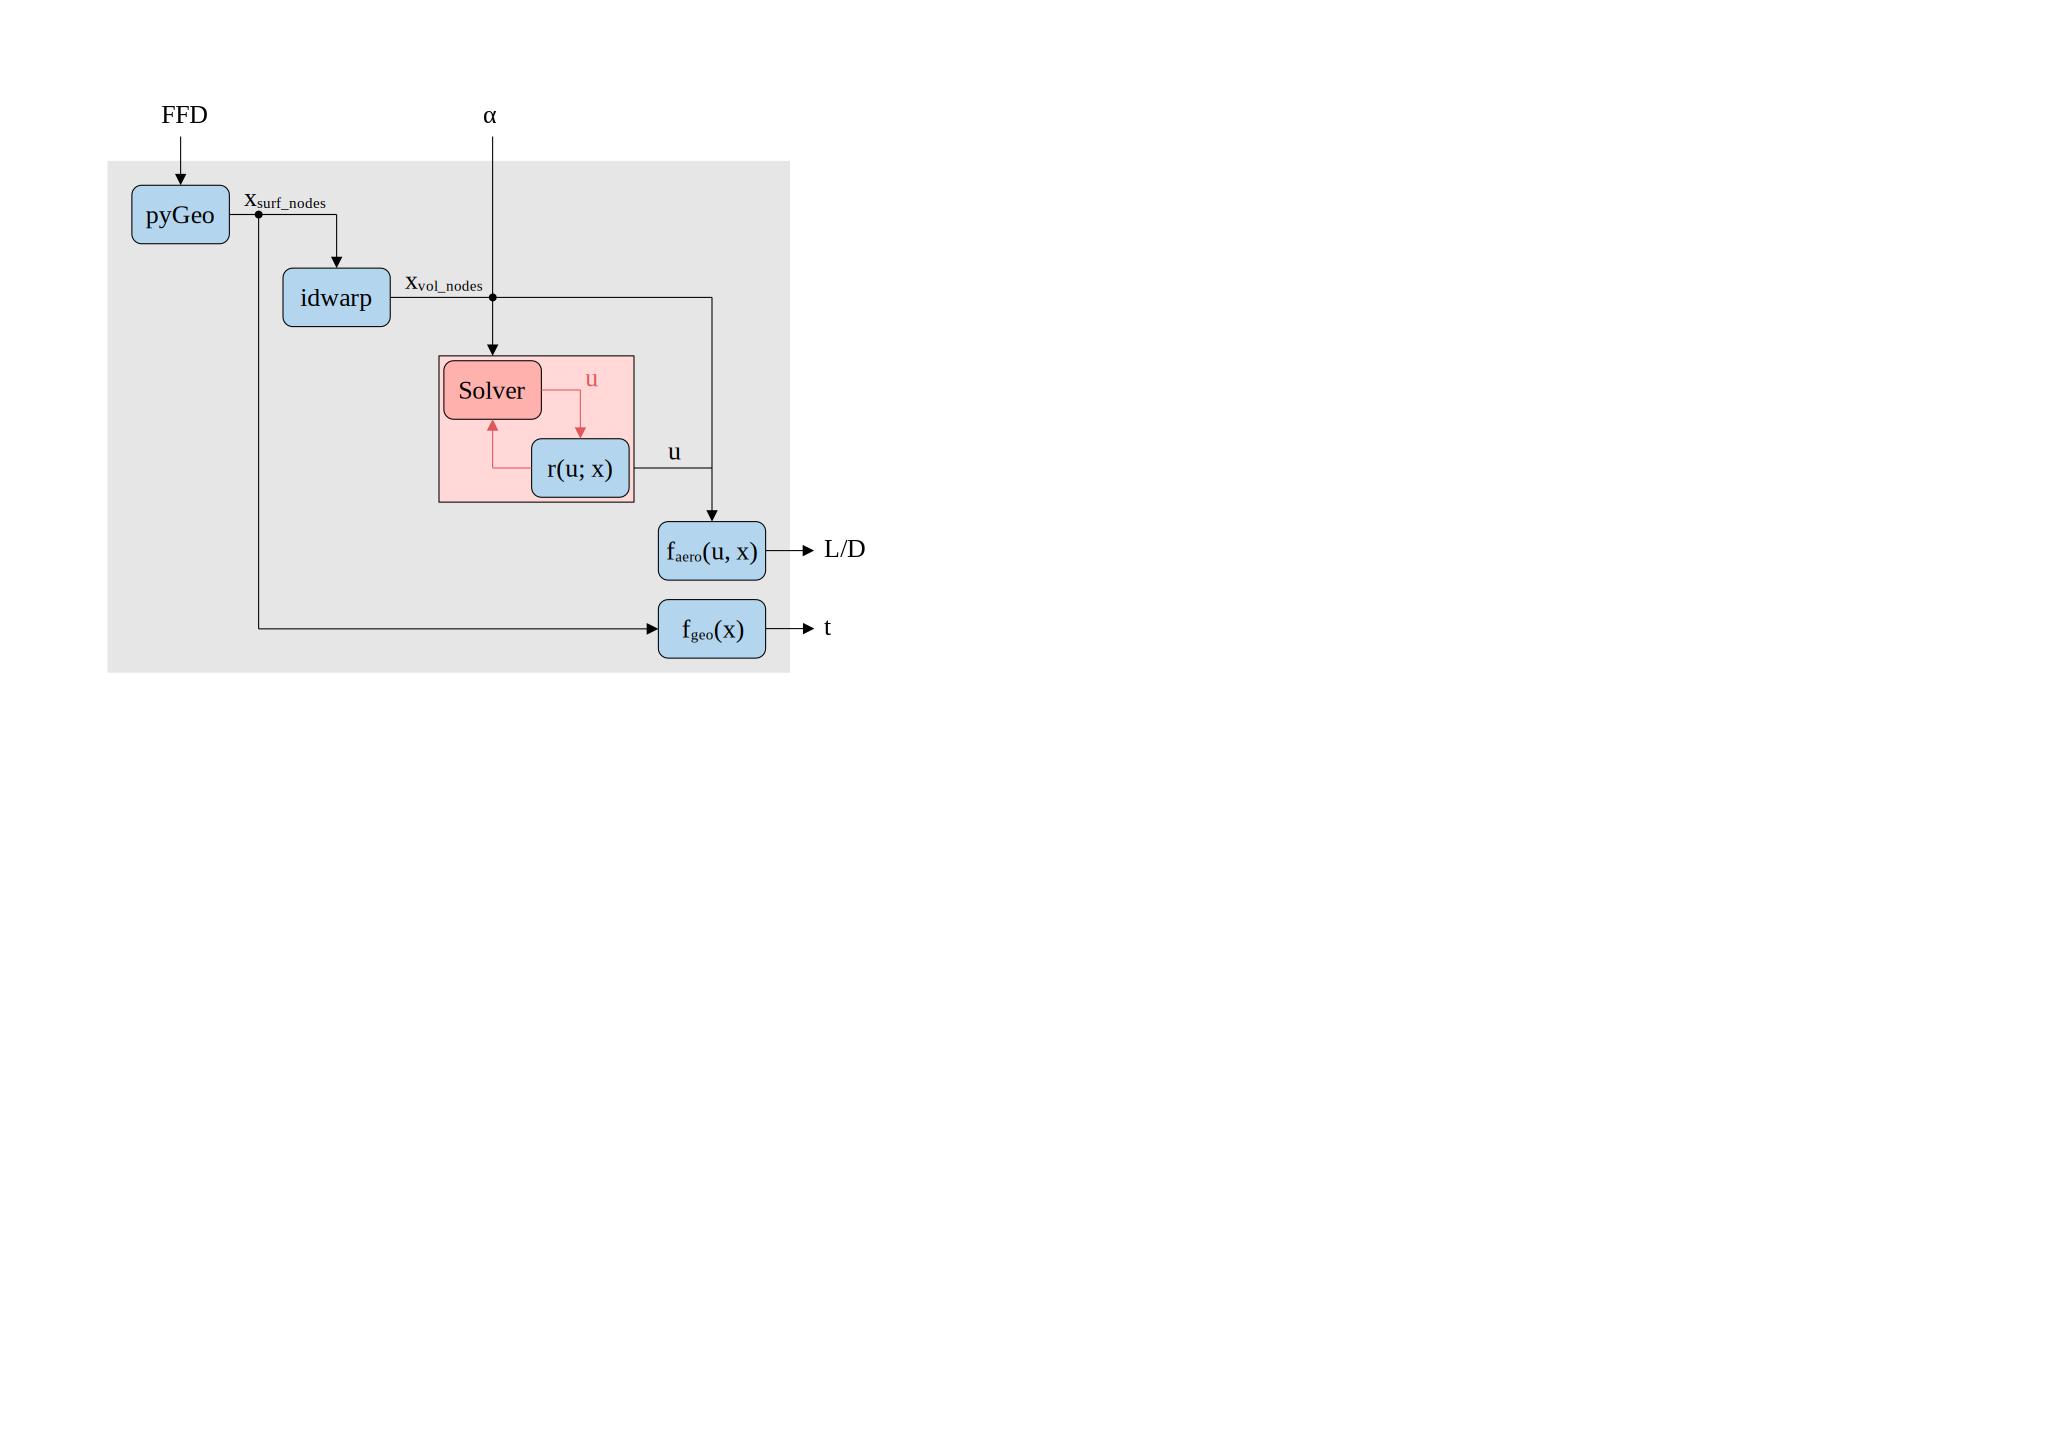
\includegraphics[width=0.7\textwidth]{MACH}
    \caption{Gradient computation dataflow in the MACH-framework. \cite{cm1}}
    \label{fig:MACH}
\end{figure}


\noindent At the top left, we have the design variables (DVs) and at the bottom
right are the functions of interest (FoI). We have two types of design
variables: \textit{aerodynamic} (such as angle of attack) and \textit{geometric
ones}. The geometry is parameterized using the \textit{Free Form Deformation
(FFD)} approach. A similar picture emerges for the FoIs: the area ($A$) of the
airfoil does only depend on the geometry, not the flow solution. But the lift
to drag ratio ($L/D$) does depend on the aerodynamic solution.

Now, lets look at the flow of data through the CFD solver. First, the
geometric DVs flow into a package called \textit{pyGeo}. It maps the FFD
variables to the surface mesh. This surface mesh is then used to warp the total
volume mesh in \textit{idwarp}. The deformed volume mesh is then feed into
ADflow where the flow solution is computed. Here, the aerodynamic DVs start to
play a role. After that, the flow variables are integrated as desired and the
final function of interest (in this case $L/D$) is assembled. As said before,
the area ($A$) does not depend on the flow solution and is directly computed
using only the surface mesh.

If you reverse the flow of information and exchange "CFD solver" with "adjoint
solver", you know how ADflow computes the total derivatives for optimization. If
you would like to learn more about it, take a look at \cite{cm1} or
\cite{mdobook}.




\subsection{Residual derivatives}
Almost all solvers mentioned need the derivative of the residuals with respect
to state variables: $r'(u) = \partial r / \partial u$. It is possible to
compute it using AD or FD. If it is done through AD, it is called
\textit{automatic differentiated pre-conditioner (ADPC)}, otherwise its called
\textit{FDPC}. Counter-intuitively, the FD pre-conditioner is more efficient
than the AD one. But the accuracy of FD is worse.

It is important to realize that this Jacobian ($\partial r / \partial u$) is
mostly zero. This is because a certain cell only depends on its neighboring
cells (and not the whole domain). This realization allows to use the concept of
coloring which is basically exploiting this non-dependence to compute most of
the derivatives in parallel. \cite{mdobook}




\subsection{Initial state of SST}
When sumb was initially developed, multiple different turbulence models
were implemented such as Spalart-Allmaras (SA) or SST. When the code was
overhauled for optimization, only the SA model was carried over and
differentiated. At that point SST would throw NaNs\footnote{Not a Number} and
crash. Lately, this was fixed to a point where the DADI turbulence solver would
work \footnote{See pull request:
\url{https://github.com/mdolab/adflow/pull/107}}. To summarize, before this
project started, the code for SST was there and a solution could be obtained
using ANK/SANK and the decoupled DADI turbulence solver. But nothing was
differentiated which means, the adjoint, NK, CANK and ANK-turb solvers were not
usable.








\section{Needed changes}
ADflow may be run in parallel where the computation is divided over multiple
cpus and computers. It does this by splitting up the computational domain into
blocks. These blocks may live on different cpus or computers. As those blocks
do not live in isolation and do depended on each other, adjacent blocks need to
exchange information. ADflow uses the \textit{halo cell} approach for this. The
idea is to have imaginary ghost (halo) cells around each block. Then they are
filled with the values from the adjacent blocks. Figure \ref{fig:halo_cells}
shows this idea. ADflow uses a second order discretizations for some terms and
thus needs two layers of halo cells.

\begin{figure}[H] \centering
\includegraphics[width=0.7\textwidth]{halo_cells}
    \caption{A block split in 4 (left) and its corresponding halo cells (right)
            \cite{cfd_halo}.}
    \label{fig:halo_cells}
\end{figure}




\subsection{Halo exchange and AD}
If one does not care about AD, this halo exchange is straight forward. But we
do, and as such, some things need to be considered. The exchange is performed
using the \textit{Message Passing Interface (MPI)}. Unfortunately, tapenade can
not handle MPI calls. To make this work, the differentiated code is divided
into two parts: The \textbf{math heavy} part is differentiated using tapenade
and the \textbf{remaining part} is hand-differentiated. This is feasible
because the hand-differentiated part consists mostly of calling the AD part and
performing communication. 

The turbulence model is considered a math heavy part that is automatically
differentiated using tapenade. For SA, this was straight forward as there is no
communication going on. But SST has one special case: The blending function
$\mathbf{F_1}$ (equation \ref{eq:f1}). For reasons that are explained later,
its value is required in halo cells. It is important to realize that halo cells
are basically clones of other compute cells in other blocks. This has been
exploited for $F_1$ by means of only computing it once and performing a halo
exchange.

Exchanging values is absolutely detrimental and ADflow has routines and places
where it is performed. But those routines are chosen carefully to not
interfere with AD. The problem with $F_1$ is the fact, that it is not a regular
flow or turbulence variable and thus, it has no such official routines for
exchange. In the legacy implementation of SST, it was just exchanged in the
model itself. But we cant do this anymore and thus the question is: Why was it
done this way and how do we get rid of this intermediate communication?

The first part of the questions might be explained by fact that sumb was
initially developed in the early 2000's. Back then, computing power was more
expensive and computing the same $F_1$ value on different blocks was
wasteful. The cost of communication was negligible in comparison. This did not
really change, but computing power became a lot cheaper. So if it makes AD
easier, it is a good trade to get rid of the communication.








\section{Changes to wall distance}
We settled on the idea of computing $F_1$ in the halo cells instead of
communicating it across. To do this, we need to take a closer look at $F_1$. It
depends on $arg_1$ (eq. \ref{eq:arg1}) which also depends on $CD_{kw}$ (eq.
\ref{eq:cdkw}). This is a bit problematic as it requires the derivatives
$\nabla k \nabla \omega$. These derivatives are discretized and thus even
more halo cells are needed to compute the halo cells. Luckily, ADflow employs
only a first-order discretization for the turbulence model. Thus, the second
layer of halo cells is enough to compute $CD_{kw}$ in the first halo layer.

On further examination, we realize that $arg_1$ also depends on the distance to
the nearest wall. Unfortunately, in ADflow, the distance to the nearest wall is
not assigned nor exchanged for halo cells . Therefor, this is the first thing
that needs to be changed.




\subsection{Wall distance computation}
Before explaining the changes, one must briefly understand how the wall
distance computation is done in ADflow. \footnote{The interested reader may
take a look at report \cite{vt1} where it is explained in more detail.} It is
important to realize that this is no easy task due to the block splitting. When
computing the distance to the nearest wall in a cell on processor X, it is
possible that the nearest wall lives on processor Y. 

To make a long story short, ADflow first determines which surface cell includes
the closets point for the current cell. This information is exchanged on
initialization and assumed to not change\footnote{This is only partially true
in the context of deforming meshes.}. After a mesh has been deformed, a
function named \texttt{updateWallDistancesQuickly()} is called. It actually
computes the distance to the earlier determined nearest surface cell. Take a
look at \cite{cm1} where this procedure is explained in more detail.




\subsection{Halo exchange}
Now, we need to quickly talk about the halo exchange routine. ADflow has two
options: \texttt{whalo1(...)} and \texttt{whalo2(...)}. The only difference
between those functions is that the first one only exchanges the halos in the
first layer and the second one exchanges all layers. For brevity, the arguments
were omitted. But they are just boolean flags that determine what variables
need to be exchanged (e.g. flow variables). We do not need the wall distance on
both halo layers. But to be future-prove,  the function \texttt{whalo2(...)}
was extended.

This extension has been straight forward. Please note that some special care
for the hand-differentiated part was needed. This is to make sure that the
derivatives are aggregated correctly in the AD part of the code. Unfortunately
(see section \ref{sec:total_derivs}), there seems to be a bug present. Because
of that, the author is not confident on how it is done best and does not
elaborate further.




\subsection{Bringing it together}
The easy approach would be to simply call \texttt{whalo2(...)} at the end of
\texttt{updateWallDistancesQuickly()}. This is not possible as this function is
AD-ed and tapenade can not handle MPI-calls. So the next obvious choice is to
call \texttt{whalo2(...)} manually every time
\texttt{updateWallDistancesQuickly()} was executed. When initializing, the
distance is computed before the communication part is initialized and thus
crashes. The final solution has been to introduce a boolean flag:
\texttt{exchangeWallDistanceHalos}. If it is true, the normal halo
exchange-calls perform also the wall distance exchange. This works fine, but is
a bit of a hack. The author believes it is possible to get rid of that flag
once he understands the code better.








\section{Algorithmic/Automatic Differentiation}
\label{sec:ad}
Once the distance to the nearest wall was available in halo cells, the
communication in $F_1$ has been removed. This paved the way to AD the whole
SST. Before explaining those changes, one must know that ADflow employs three
different versions of differentiated code: \textit{forwards},
\textit{backwards} and \textit{backwards\_fast}. 

The first two modes are the regular AD approaches. The \textit{backwards\_fast}
routine is a striped down version of the normal \textit{backwards} routine
which is done for performance reasons. Table \ref{tab:ad_routines} gives an
overview on where what routine may be used. If multiple options are available,
only one is enough.

\begin{table}[H]
    \centering
    \begin{tabular}{l c c c}
        \toprule
                                            & forwards  & backwards     & 
                                            backwards\_fast \\
        \midrule
        Assemble $\partial r / \partial u$  &  X        &               & X \\ 
        Compute total derivatives           &           & X             &   \\
        ADPC for ANK                        &  X        &               &   \\
        ADPC for NK                         &  X        &               &   \\
        \bottomrule
    \end{tabular}
    \caption{When what AD routines are used in ADflow.}
    \label{tab:ad_routines}
\end{table}

\noindent It becomes clear that the forwards routine is the most important one.
It allows to use almost all features except for total derivative computation.
But once this is implemented, the reverse routines are not much more effort.
The reverse\_fast routines are great to speed up the computation but are not
needed for a first running prototype.




\subsection{Implementation}
In order to AD the SST code, the following procedure has been followed:

\begin{enumerate}
    \item Split the whole code in two parts: part (a) computes the residuals
        and part (b) solves SST in a decoupled manner using DADI. 

    \item Part (b) stays as it is but needs to be called in the right spot.

    \item Part (a) is split up even more: (I) compute $kw_{cd}$, (II) compute
        $F_1$, (III) compute the production terms, (IV) compute the source
        terms, (V) compute the advection term, (VI) compute the unsteady term,
        (VII) compute the viscous terms and finally (VIII) scale the residuals.

    \item AD the sub-parts I through VIII using the forward routines. 

    \item Verify the forwards routines (see sec. \ref{subsubsec:forward_ad}).

    \item AD the sub-parts I through VIII using the backwards routines.

    \item Verify the backwards routines (see sec. \ref{subsubsec:backwards_ad}).

    \item AD the sub-parts I through VIII using the backwards\_fast routines.

    \item Verify the backwards\_fast routines (see sec.
        \ref{subsubsec:backwards_fast_ad}).
\end{enumerate}

\noindent When looking at the routine that computes $F_1$ (II), one has to take
special care: To compute $F_1$, we need the distance to the nearest wall. This
has been fixed for regular halo cells and works as intended, but this distance
is not defined for halo cells that lie behind a boundary condition (like a
wall). The legacy implementation solves this as follows:

\begin{enumerate}
    \item allocate $F_1$ on all halo cells (including boundary conditions (BC))

    \item compute $F_1$ on all cells (including BCs).

    \item Loop over halos that lie behind a BC and simply copy the $F_1$ value
        from the nearest compute cell. This effectively is a \textit{Neumann
        boundary condition}.
\end{enumerate}

\noindent This procedure works fine for the regular residual evaluation. It
also works for the forward AD mode. But when looking at the reverse mode, one
has to reverse the procedure mentioned: first we apply the Neumann BC (3), and
then (2) we overwrite $F_1$ with garbage that depends on an un-initialized wall
distance. To prevent this, we must take special care to not loop over BC halos
in step (2).








\section{Verification}
This section explains how SST and its derivatives were verified.




\subsection{Testcases for robustness}
To make sure, SST and the various solvers work under different circumstances,
two testcases were set up. They are also used to show that the
modifications made in this project did not change the legacy SST implementation
that was available at the beginning.


\subsubsection{NACA 0012}
This first testcase is a NACA0012 airfoil under a low angle of attack and mach
number. The mesh is a bit to coarse to obtain a physical solution. But this has
the advantage that the solution is obtained faster. Which allows it to be used
for debugging. Table \ref{tab:flow_conditions_n0012} lists the flow conditions
and table \ref{tab:mesh_parameters_n0012} lists the mesh parameters.

\begin{table}[H]
    \centering
    \begin{tabular}{l r}
        \toprule
        Parameter                           & Value \\
        \midrule
        Angle of Attack                     & $3 \degree$ \\
        Reynolds number                     & $5e6$ \\
        Mach number                         & $0.3$ \\
        Temperature                         & $288 \degree K$\\
        \bottomrule
    \end{tabular}
    \caption{Flow conditions for the NACA0012 testcase.}
    \label{tab:flow_conditions_n0012}
\end{table}

\begin{table}[H]
    \centering
    \begin{tabular}{l r}
        \toprule
        Parameter                           & Value \\
        \midrule
        Chord length                        & $1$ \\
        Farfield distance                   & $100$ \\
        dimensional wall distance           & $3e-6$ \\
        Growth ratio                        & $\sim 1.05$ \\
        Points on airfoil surface           & $245$\\
        Points normal to flow direction     & $129$ \\
        Number of compute cells             & $31'232$\\
        \bottomrule
    \end{tabular}
    \caption{Mesh parameters for the NACA0012 testcase.}
    \label{tab:mesh_parameters_n0012}
\end{table}


\subsubsection{RAE 2822}
This setup uses the supercritical RAE 2822 airfoil. As such, it operates in the
transsonic regime which is dominated by mach effects and shocks. Table
\ref{tab:mesh_parameters_rae2822} lists the mesh parameters and table
\ref{tab:flow_conditions_rae2822} the flow conditions. Similar to the NACA
testcase, the number of compute cells is to low to obtain physical correct
results. 

\begin{table}[H]
    \centering
    \begin{tabular}{l r}
        \toprule
        Parameter                           & Value \\
        \midrule
        Angle of Attack                     & $2.92 \degree$ \\
        Reynolds number                     & $6.5e6$ \\
        Mach number                         & $0.725$ \\
        Temperature                         & $288 \degree K$\\
        \bottomrule
    \end{tabular}
    \caption{Flow conditions for RAE2822 testcase.}
    \label{tab:flow_conditions_rae2822}
\end{table}

\begin{table}[H]
    \centering
    \begin{tabular}{l r}
        \toprule
        Parameter                           & Value \\
        \midrule
        Chord length                        & $1$ \\
        Farfield distance                   & $100$ \\
        dimensional wall distance           & $3e-6$ \\
        Growth ratio                        & $\sim 1.05$ \\
        Points on airfoil surface           & $129$\\
        Points normal to flow direction     & $129$ \\
        Number of compute cells             & $16'384$\\
        \bottomrule
    \end{tabular}
    \caption{Mesh parameters for RAE2822 testcase.}
    \label{tab:mesh_parameters_rae2822}
\end{table}




\subsection{Testcases for accuracy}
The following testcases were primarily setup to make sure SST is implemented
correctly. Of course, they also provide a way to test the solvers under
different circumstances.


\subsubsection{Flatplate}
The flatplate at zero incidence is a classic testcase for basic flow
experiments and CFD solver verification. The setup and meshes were provided
by a website called \textit{Turbulence Modeling Resource (TMR)} which is
maintained by NASA. Figure \ref{fig:plate_bc} shows the flow setup and table
\ref{tab:plate_mesh_sizes} list the number of cells per grid-level. All grids
were obtained from that TMR website.

\begin{figure}[H] \centering
    \includegraphics[width=0.8\textwidth]{plate_bc}
    \caption{Boundary conditions and test case overview. \cite{nasatmr}}
    \label{fig:plate_bc}
\end{figure}

\begin{table}[H]
    \centering
    \begin{tabular}{c r r}
        \toprule
        Identifier      & \# of nodes   & \# of cells \\
        \midrule
        L4              & 1'800         & 816 \\
        L3              & 6'860         & 3'264 \\
        L2              & 26'772        & 13'056 \\
        L1              & 105'764       & 52'224 \\
        L0              & 420'420       & 208'896 \\
        \bottomrule
    \end{tabular}
    \caption{Mesh sizes used for the flatplate testcases.}
    \label{tab:plate_mesh_sizes}
\end{table}


\subsubsection{2D bump}
This is also a classic testcase and as such is also provided by the TMR
website. It is more involved and harder to simulate as it contains an adverse
pressure gradient after the bump. Figure \ref{fig:2dbump_bc} shows the boundary
conditions, figure \ref{fig:2dbump_closeup} gives a close up of the bump and
tab. \ref{tab:2dbump_mesh_sizes} lists the mesh sizes.

\begin{figure}[H] \centering
    \includegraphics[width=0.6\textwidth]{2dbump_bc_overview.jpg}
    \caption{2D bump test case overview. \cite{nasatmr}}
    \label{fig:2dbump_bc}
\end{figure}

\begin{figure}[H] \centering
    \includegraphics[width=0.7\textwidth]{2dbump_bc_closeup.jpg}
    \caption{Close up of 2D bump. \cite{nasatmr}}
    \label{fig:2dbump_closeup}
\end{figure}

\begin{table}[H]
    \centering
    \begin{tabular}{c r r}
        \toprule
        Identifier      & \# of nodes   & \# of cells \\
        \midrule
        L4              & 7'462         & 3'520 \\
        L3              & 28'998        & 14'080 \\
        L2              & 114'310       & 56'320\\
        L1              & 453'894       & 225'280 \\
        L0              & 1'808'902     & 901'120 \\
        \bottomrule
    \end{tabular}
    \caption{Mesh sizes used for the 2D bump testcase.}
    \label{tab:2dbump_mesh_sizes}
\end{table}




\subsection{Testcases for derivatives}
\subsubsection{3D wing}
This is the only 3D test employed. It makes sure the changes also work in the
third dimension, but it is primarily intended for gradient verification. It is
quite coarse and thus not physical. Figure \ref{fig:3dwing_setup} shows the
surface mesh with its \textit{Free Form Deformation (FFD)} points around. They
are used as a parametrisation for various geometric design variables. Table
\ref{tab:3dwing_flowconditions} lists the flow conditions and table
\ref{tab:3dwing_dvs} shows the design variables available.

\begin{figure}[H] \centering
    \includegraphics[width=\textwidth]{test_setup}
    \caption{Surface mesh (blue) and FFD points (green) for the automated test
    setup. \cite{vt1}}
    \label{fig:3dwing_setup}
\end{figure}

\begin{table}[H]
    \centering
    \begin{tabular}{l l l}
        \toprule
        Name  & Type & Comment \\
        \toprule
        shape   & geometric   & Local pertubations of FFD points. \\
        twist   & geometric   & Twisting of wing at each FFD-section. \\
        span    & geometric   & Length of the wing. \\
        alpha   & aerodynamic & Angle of attack. \\
        beta    & aerodynamic & Slip angle. \\
        mach    & aerodynamic & Mach number. \\
        P       & aerodynamic & Pressure. \\
        T       & aerodynamic & Temperature. \\
        xRef    & aerodynamic & X location of reference point for moment
        calculation \\
        yRef    & aerodynamic & Y location of reference point for moment
        calculation \\
        zRef    & aerodynamic & Z location of reference point for moment
        calculation \\
        \bottomrule
    \end{tabular}
    \caption{Design variables for the 3D wing testcase.\label{tab:3dwing_dvs}}
\end{table}

\begin{table}[H]
    \centering
    \begin{tabular}{l r}
        \toprule
        Parameter               & Value \\
        \midrule
        Specific gas constant   & $287.87 J / (kg K)$ \\
        Pressure                & $200 hPa$ \\
        Temperature             & $220 \degree K$ \\
        Alpha                   & $1.8 \degree$ \\
        Mach                    & $0.8$ \\
        Mesh node count         & $30'375$ \\
        Mesh cell count         & $24'192$ \\
        \bottomrule
    \end{tabular}
    \caption{Flow conditions for the automated test setup.}
    \label{tab:3dwing_flowconditions}
\end{table}




\subsection{Partial derivatives}
To verify any derivative in this report, the before mentioned 3D wing testcase
is used. ADflow computes the following partial derivatives:

\begin{align}
    &\frac{\partial r}{\partial u}& \qquad 
    &\frac{\partial f}{\partial u}& \qquad
    &\frac{\partial F}{\partial u}& \qquad \\
%
    &\frac{\partial r}{\partial x_{geo}}& \qquad  
    &\frac{\partial f}{\partial x_{geo}}& \qquad
    &\frac{\partial F}{\partial x_{geo}}&\qquad \\
%
    &\frac{\partial r}{\partial x_{aero}}& \qquad  
    &\frac{\partial f}{\partial x_{aero}}& \qquad
    &\frac{\partial F}{\partial x_{aero}}& \qquad \\
\end{align}

\noindent Where $r$ are the residuals, $u$ the state variables, $f$ the
functions of interest and $F$ the forces on the nodes of the mesh. $x$ are the
geometric or aerodynamic design variables (see sec. \ref{subsec:adjoint}). All
those partial derivatives are obtained using either forward or backwards AD
mode.


As explained in sec. \ref{sec:ad}, the \textit{backwards\_fast} mode is a
subset and only provides:
\begin{equation}
    \frac{\partial r}{\partial u}
\end{equation}


\subsubsection{Verification}
To verify the various derivatives, the following procedure is followed:

\begin{enumerate}
    \item Verify forward partials against finite differences.

    \item Verify the forward partials against complex step.

    \item Verify the backwards partials against the forward ones using the
        dot-product test.

    \item Verify the backwards\_fast partials against the regular backwards
        partial derivatives.
\end{enumerate}




\subsection{Total derivatives}
\label{subsec:total_derivs}
Verifying the total derivatives is more straight forward using the 3D wing
testcase. First, we obtain accurate total derivatives using complex step. Then
we compute them using the adjoint approach. Please note that there are two ways
to assemble the state residual matrix ($\partial r / \partial u$): either by
using the forward AD or backwards\_fast AD mode. Finally, we need to compare
all derivatives and make sure they match to a reasonable tolerance.




\subsection{Regression tests}
\noindent ADflow uses regression tests to make sure new features do not break
existing ones. Those test usually use the 3D wing testcase under the hood and
have been extended for SST. Table \ref{tab:automated_tests} lists what tests
have been extended and what they are used for.

\begin{table}[H]
    \centering
    \begin{tabular}{l p{0.7\textwidth}}
        \toprule
        Name                                & Purpose \\
        \midrule
        \texttt{test\_jacVecProdFWD.py}     & Makes sure the partial
            derivatives agree to FD and CS. It basically performs step (1) and
            (2) from the previous section.\\

        \texttt{test\_functionals.py}       & This tests a lot of different
            things. But we are mostly interested in the dot-product test that
            makes sure forward AD is consistent with backwards AD. It is
            basically step (3). \\

        \texttt{test\_jacVecProdBWDFast.py} & This test makes sure the
            backwards\_fast AD routines agree with the backwards AD routines. \\

        \texttt{test\_adjoint.py}            & Makes sure the total derivatives
            agree with derivatives obtained using complex step. \\
        \bottomrule
    \end{tabular}
    \caption{Automated test setup.}
    \label{tab:automated_tests}
\end{table}



